\chapter{验证数据与可复现实验}
\label{app:validation}
\section{自动化测试}
本次验证运行的 137 项测试全部通过，包含真实 MCP 标准输入输出初始化、工具列举和调用，未跳过该传输测试。运行使用 Python 3.12、NumPy 2.3.5、SciPy 1.17.0、Gemmi 0.7.5、Matplotlib 3.10.8、Plotly 7.1.0、scikit-image 0.26.0 和 MCP SDK 2.3.0。

测试包括晶胞和距离的解析或独立计算、六类空间群的结构因子对照、230 个参考空间群的系统消光、特殊位置与张量、异常散射、负强度、各种参数化、秩缺失、反射分组、格式往返、Fourier 地图、概率椭球和运行记录。测试通过表示这些明确断言成立，不意味着所有可能结构或官方指令都已被覆盖。

\begin{lstlisting}
python -m pip install -e ".[dev,mcp]"
ARIADNE_MCP_STDIO_TEST=1 python -m pytest -q
python -m ruff check src tests
\end{lstlisting}
MCP 传输测试需要运行环境允许本地进程和事件循环通信；默认测试将该项作为可选项。本次已经在允许相应通信的环境中实际执行。没有使用外部 LLM 账号或远程模型调用来替代传输测试。

\section{解析与独立实现对照}
单参数尺度检验使用式~\eqref{eq:scaleclosed}，负强度参与分子求和，结果及标准不确定度应与优化器一致。特殊位置检验对唯一对称位置求和，防止多重计数。张量检验比较式~\eqref{eq:ucif} 转换前后的散射指数。Fourier 检验用单个已知位置和直接求和检验峰方向、体积归一化和周期边界。概率椭球检验直接回代式~\eqref{eq:ellipsoid}。

Gemmi 独立结构因子计算用于检验原生求和，包括非正交晶胞与各向异性位移。Gemmi 同时提供本实现使用的标准表格，因此这些对照能检验求和、变换和约定，但不能独立验证散射表本身。散射表采用公开标准数据~\cite{gemmi_scattering,gemmi_symmetry}。

\section{从幅度到坐标的完整合成恢复}
四个碳原子置于 $a=5.2$、$b=5.7$、$c=6.1\,\angstrom$ 的正交 $P1$ 晶胞中，分数坐标为
\begin{equation}
\begin{pmatrix}
0.113&0.239&0.337\\
0.371&0.628&0.793\\
0.725&0.159&0.563\\
0.842&0.771&0.188
\end{pmatrix},\qquad U_{\mathrm{iso}}=0.012\,\angstrom^2.
\end{equation}
使用 4540 条合成反射，选择条件为 $d>0.55\,\angstrom$。未叠加随机噪声，$\sigma=0.2$ 仅用于目标尺度。求解器只接收晶胞、四个碳元素、强度和标准差，不接收真值坐标。随机种子为 1729，共 4 个起点，每个 400 次迭代。

\begin{table}[htbp]\centering\small
\begin{tabular}{rrrr}
\toprule 候选 & 精修前 RMS/$\angstrom$ & 精修后 RMS/$\angstrom$ & 精修后 $wR_2$\\\midrule
1&0.015254&$1.56\times10^{-16}$&$1.36\times10^{-15}$\\
2&0.013536&$4.00\times10^{-16}$&$1.44\times10^{-15}$\\
3&0.011407&$5.99\times10^{-16}$&$1.46\times10^{-15}$\\
4&0.010608&$8.69\times10^{-17}$&$1.33\times10^{-15}$\\
\bottomrule
\end{tabular}
\caption{同一合成数据的四个相位起点。RMS 在共同原点平移、反演与同元素原子排列优化后计算。}
\end{table}
这项实验验证了该实例的求解与精修链路。机器精度级残差来自无噪声数据和匹配的正向模型，不能解释为实验坐标精度，更不能外推为复杂结构的解析成功率。复现脚本为 \code{validation/run_phasing_recovery.py}，全部输入、候选和结果一并提供。

\section{有噪声数据与未参与拟合的反射}
交互绘图示例是一个明确标识的合成重原子模型，包含 10 个原子和非正交晶胞，其中 Br 采用各向异性位移。4446 条反射按固定种子产生独立高斯噪声，标准差为
\begin{equation}
\sigma_h=\sqrt{4+I_h^{\mathrm{true}}}+0.01I_h^{\mathrm{true}}.
\end{equation}
按对称与 Friedel 轨道预先留出 446 条，4000 条用于拟合，共 43 个独立参数。所得工作集 $R_1=0.018754$、$wR_2=0.046004$、$S=0.992143$；留出集 $wR_2=0.043572$。Jacobian 秩为 43/43。该示例演示输入快照、独立分组、精修、地图和离线绘图的完整调用，数据生成脚本与种子均包含在源码包内。

\section{公开 \texorpdfstring{FeN$_4$}{FeN4} 实测数据重新精修}
公开实验来自 Bykov 等人的 FeN$_4$ 研究~\cite{fen4_2018}。原始数据为高压单晶衍射，归档结构属于 $P\bar1$，不对称单元含 3 个原子，其中 Fe 位于反演中心。验证使用归档结构因子 CIF 中的 71 个实测 $F^2$ 与标准差；没有把同文件中的计算强度列作为观测。

采用归档给出的各向同性位移模型、显式异常散射修正和权重 $a=0.0282$、$b=0.3122$；晶胞使用结构因子文件中保留更多小数位的数值。Fe 坐标由反演中心固定，其他位置、各向同性位移与尺度构成 10 个独立参数。

\begin{table}[htbp]\centering\small
\begin{tabular}{lrr}
\toprule 指标 & 原生重新精修 & 公开归档值\\\midrule
$R_1[I>2\sigma(I)]$ & 0.04031574947 & 0.0403\\
$R_1$，全部反射 & 0.04126821960 & 0.0413\\
$wR_2$ & 0.08148047295 & 0.0815\\
拟合优度 $S$ & 1.183324413 & 1.183\\
Jacobian 秩/参数数 & 10/10 & 10 个参数\\
\bottomrule
\end{tabular}
\caption{原生精修复现公开归档指标的报告精度。相同的公开观测用于两列指标；本次未运行官方二进制程序。}
\end{table}
将初始 N 坐标扰动约 0.02 个分数坐标，并改变一个位移参数后，再次精修所得坐标与第一结果最大相差约 $5.1\times10^{-10}$。这说明该实例的结果不是单纯读取归档坐标或残差数值，而是通过重新优化恢复。

\begin{figure}[htbp]
\centering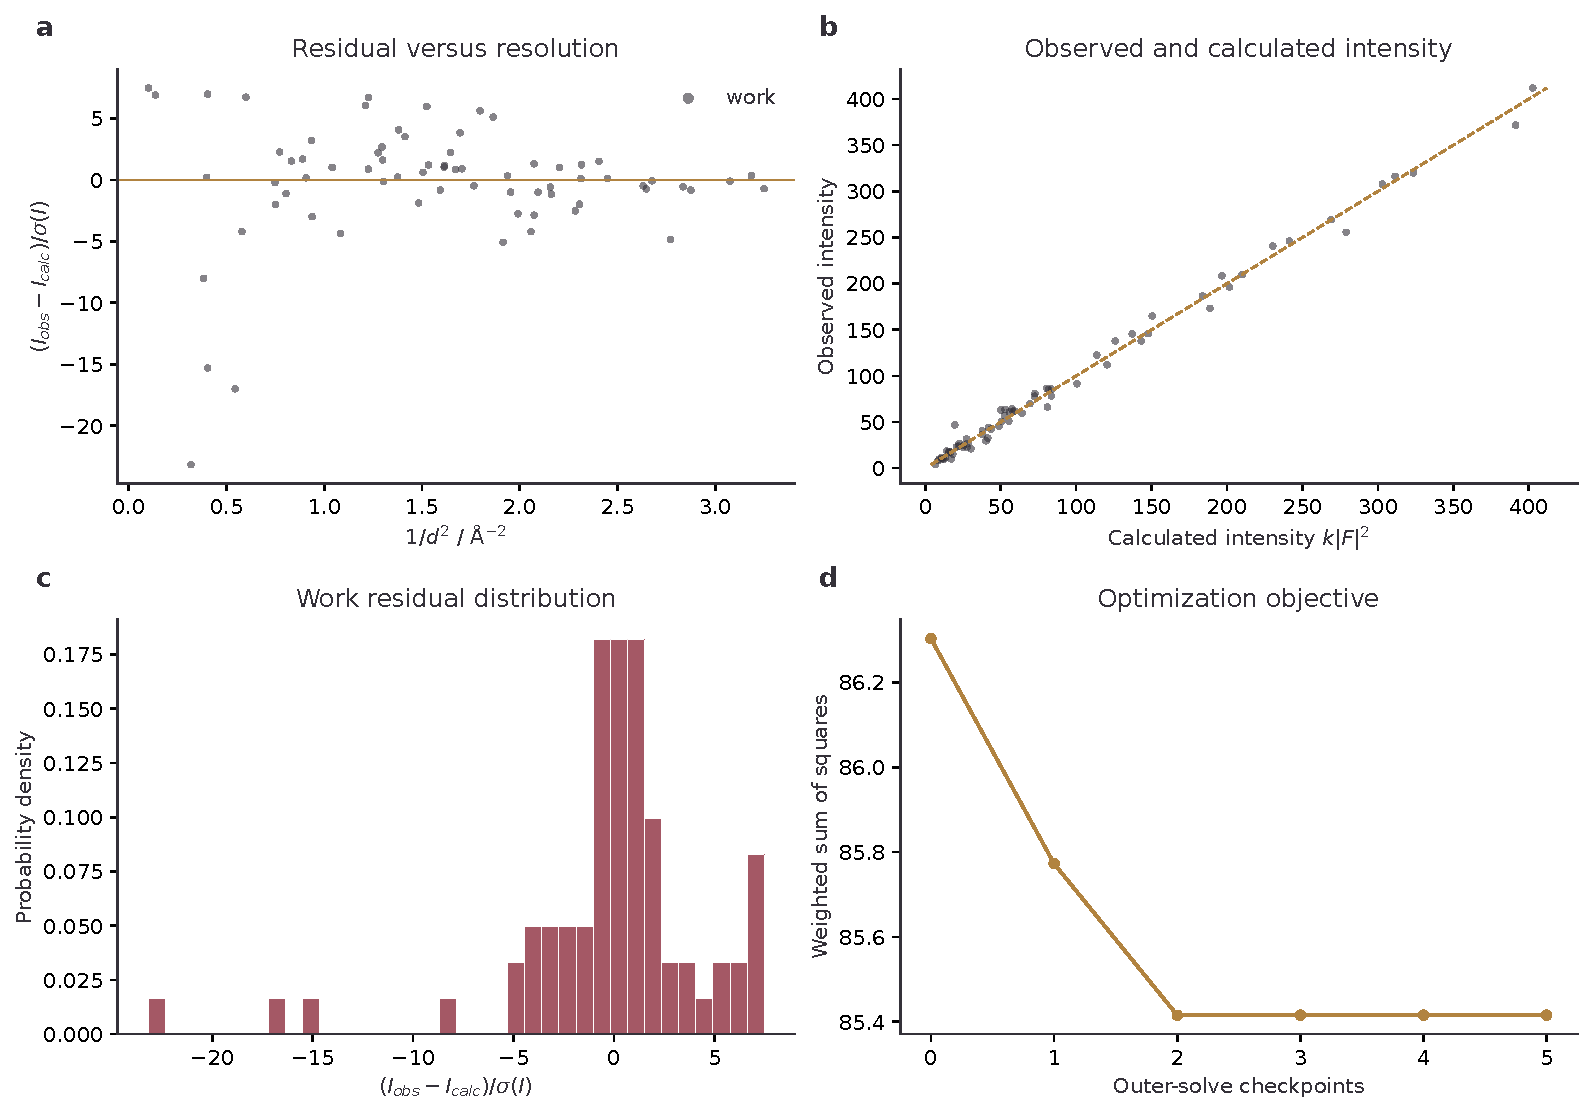
\includegraphics[width=\textwidth]{figures/fen4_refinement_diagnostics.pdf}
\caption{FeN$_4$ 的公开实测数据诊断。该例检验已知结构的精修，不构成从零求相位、运行速度或全部化学体系的基准。}
\end{figure}

原始 CIF、反射 CIF、文章引用、下载来源、许可说明与 SHA-256 均位于 \code{validation/public_data/}。脚本 \code{validation/run_real_fen4.py} 明确选择实测列、晶胞精度和权重，并保存完整机器结果。

\section{验证结论的适用范围}
当前证据支持：所列核心数学约定一致；已测例中的结构因子与约束精修正确；公开 FeN$_4$ 指标可复现；指定 $P1$ 合成结构能从幅度恢复；agent 请求可归档并通过实际 MCP 传输执行。尚没有开展完整官方二进制对照、多化学体系成功率研究或与 SHELXT/SHELXL 的等条件速度比较。上述验证与能力表共同界定本次交付，而不互相替代。
